\documentclass[twoside]{book}

% Packages required by doxygen
\usepackage{fixltx2e}
\usepackage{calc}
\usepackage{doxygen}
\usepackage[export]{adjustbox} % also loads graphicx
\usepackage{graphicx}
\usepackage[utf8]{inputenc}
\usepackage{makeidx}
\usepackage{multicol}
\usepackage{multirow}
\PassOptionsToPackage{warn}{textcomp}
\usepackage{textcomp}
\usepackage[nointegrals]{wasysym}
\usepackage[table]{xcolor}

% Font selection
\usepackage[T1]{fontenc}
\usepackage[scaled=.90]{helvet}
\usepackage{courier}
\usepackage{amssymb}
\usepackage{sectsty}
\renewcommand{\familydefault}{\sfdefault}
\allsectionsfont{%
  \fontseries{bc}\selectfont%
  \color{darkgray}%
}
\renewcommand{\DoxyLabelFont}{%
  \fontseries{bc}\selectfont%
  \color{darkgray}%
}
\newcommand{\+}{\discretionary{\mbox{\scriptsize$\hookleftarrow$}}{}{}}

% Page & text layout
\usepackage{geometry}
\geometry{%
  a4paper,%
  top=2.5cm,%
  bottom=2.5cm,%
  left=2.5cm,%
  right=2.5cm%
}
\tolerance=750
\hfuzz=15pt
\hbadness=750
\setlength{\emergencystretch}{15pt}
\setlength{\parindent}{0cm}
\setlength{\parskip}{0.2cm}
\makeatletter
\renewcommand{\paragraph}{%
  \@startsection{paragraph}{4}{0ex}{-1.0ex}{1.0ex}{%
    \normalfont\normalsize\bfseries\SS@parafont%
  }%
}
\renewcommand{\subparagraph}{%
  \@startsection{subparagraph}{5}{0ex}{-1.0ex}{1.0ex}{%
    \normalfont\normalsize\bfseries\SS@subparafont%
  }%
}
\makeatother

% Headers & footers
\usepackage{fancyhdr}
\pagestyle{fancyplain}
\fancyhead[LE]{\fancyplain{}{\bfseries\thepage}}
\fancyhead[CE]{\fancyplain{}{}}
\fancyhead[RE]{\fancyplain{}{\bfseries\leftmark}}
\fancyhead[LO]{\fancyplain{}{\bfseries\rightmark}}
\fancyhead[CO]{\fancyplain{}{}}
\fancyhead[RO]{\fancyplain{}{\bfseries\thepage}}
\fancyfoot[LE]{\fancyplain{}{}}
\fancyfoot[CE]{\fancyplain{}{}}
\fancyfoot[RE]{\fancyplain{}{\bfseries\scriptsize Generated on Thu Aug 20 2015 00\+:10\+:48 for re\+:all Project by Doxygen }}
\fancyfoot[LO]{\fancyplain{}{\bfseries\scriptsize Generated on Thu Aug 20 2015 00\+:10\+:48 for re\+:all Project by Doxygen }}
\fancyfoot[CO]{\fancyplain{}{}}
\fancyfoot[RO]{\fancyplain{}{}}
\renewcommand{\footrulewidth}{0.4pt}
\renewcommand{\chaptermark}[1]{%
  \markboth{#1}{}%
}
\renewcommand{\sectionmark}[1]{%
  \markright{\thesection\ #1}%
}

% Indices & bibliography
\usepackage{natbib}
\usepackage[titles]{tocloft}
\setcounter{tocdepth}{3}
\setcounter{secnumdepth}{5}
\makeindex

% Hyperlinks (required, but should be loaded last)
\usepackage{ifpdf}
\ifpdf
  \usepackage[pdftex,pagebackref=true]{hyperref}
\else
  \usepackage[ps2pdf,pagebackref=true]{hyperref}
\fi
\hypersetup{%
  colorlinks=true,%
  linkcolor=blue,%
  citecolor=blue,%
  unicode%
}

% Custom commands
\newcommand{\clearemptydoublepage}{%
  \newpage{\pagestyle{empty}\cleardoublepage}%
}


%===== C O N T E N T S =====

\begin{document}

% Titlepage & ToC
\hypersetup{pageanchor=false,
             bookmarks=true,
             bookmarksnumbered=true,
             pdfencoding=unicode
            }
\pagenumbering{roman}
\begin{titlepage}
\vspace*{7cm}
\begin{center}%
{\Large re\+:all Project }\\
\vspace*{1cm}
{\large Generated by Doxygen 1.8.9.1}\\
\vspace*{0.5cm}
{\small Thu Aug 20 2015 00:10:48}\\
\end{center}
\end{titlepage}
\clearemptydoublepage
\tableofcontents
\clearemptydoublepage
\pagenumbering{arabic}
\hypersetup{pageanchor=true}

%--- Begin generated contents ---
\chapter{Hierarchical Index}
\section{Class Hierarchy}
This inheritance list is sorted roughly, but not completely, alphabetically\+:\begin{DoxyCompactList}
\item Q\+Abstract\+Graphics\+Shape\+Item\begin{DoxyCompactList}
\item \contentsline{section}{My\+Central\+Graphics\+Item}{\pageref{class_my_central_graphics_item}}{}
\begin{DoxyCompactList}
\item \contentsline{section}{My\+Central\+Ellipse\+Item}{\pageref{class_my_central_ellipse_item}}{}
\item \contentsline{section}{My\+Central\+Rect\+Item}{\pageref{class_my_central_rect_item}}{}
\item \contentsline{section}{My\+Central\+Rect\+Radious\+Item}{\pageref{class_my_central_rect_radious_item}}{}
\end{DoxyCompactList}
\item \contentsline{section}{My\+Dock\+Text\+Item}{\pageref{class_my_dock_text_item}}{}
\end{DoxyCompactList}
\item Q\+Dock\+Widget\begin{DoxyCompactList}
\item \contentsline{section}{My\+Organization\+Dock\+Widget}{\pageref{class_my_organization_dock_widget}}{}
\end{DoxyCompactList}
\item Q\+Graphics\+Ellipse\+Item\begin{DoxyCompactList}
\item \contentsline{section}{My\+Ellipse\+Item}{\pageref{class_my_ellipse_item}}{}
\end{DoxyCompactList}
\item Q\+Graphics\+Rect\+Item\begin{DoxyCompactList}
\item \contentsline{section}{My\+Rect\+Item}{\pageref{class_my_rect_item}}{}
\item \contentsline{section}{My\+Rect\+Radious\+Item}{\pageref{class_my_rect_radious_item}}{}
\end{DoxyCompactList}
\item Q\+Graphics\+Scene\begin{DoxyCompactList}
\item \contentsline{section}{My\+Drop\+Graphics\+Scene}{\pageref{class_my_drop_graphics_scene}}{}
\end{DoxyCompactList}
\item Q\+Graphics\+Text\+Item\begin{DoxyCompactList}
\item \contentsline{section}{My\+Simple\+Text\+Item}{\pageref{class_my_simple_text_item}}{}
\end{DoxyCompactList}
\item Q\+Graphics\+View\begin{DoxyCompactList}
\item \contentsline{section}{My\+Graphics\+View}{\pageref{class_my_graphics_view}}{}
\end{DoxyCompactList}
\item Q\+Main\+Window\begin{DoxyCompactList}
\item \contentsline{section}{Main\+Window}{\pageref{class_main_window}}{}
\end{DoxyCompactList}
\item Q\+Point\+F\begin{DoxyCompactList}
\item \contentsline{section}{My\+Point\+F}{\pageref{class_my_point_f}}{}
\end{DoxyCompactList}
\end{DoxyCompactList}

\chapter{Class Index}
\section{Class List}
Here are the classes, structs, unions and interfaces with brief descriptions\+:\begin{DoxyCompactList}
\item\contentsline{section}{\hyperlink{class_main_window}{Main\+Window} }{\pageref{class_main_window}}{}
\item\contentsline{section}{\hyperlink{class_my_central_ellipse_item}{My\+Central\+Ellipse\+Item} }{\pageref{class_my_central_ellipse_item}}{}
\item\contentsline{section}{\hyperlink{class_my_central_graphics_item}{My\+Central\+Graphics\+Item} }{\pageref{class_my_central_graphics_item}}{}
\item\contentsline{section}{\hyperlink{class_my_central_rect_item}{My\+Central\+Rect\+Item} }{\pageref{class_my_central_rect_item}}{}
\item\contentsline{section}{\hyperlink{class_my_central_rect_radious_item}{My\+Central\+Rect\+Radious\+Item} }{\pageref{class_my_central_rect_radious_item}}{}
\item\contentsline{section}{\hyperlink{class_my_dock_text_item}{My\+Dock\+Text\+Item} }{\pageref{class_my_dock_text_item}}{}
\item\contentsline{section}{\hyperlink{class_my_drop_graphics_scene}{My\+Drop\+Graphics\+Scene} }{\pageref{class_my_drop_graphics_scene}}{}
\item\contentsline{section}{\hyperlink{class_my_ellipse_item}{My\+Ellipse\+Item} }{\pageref{class_my_ellipse_item}}{}
\item\contentsline{section}{\hyperlink{class_my_graphics_view}{My\+Graphics\+View} }{\pageref{class_my_graphics_view}}{}
\item\contentsline{section}{\hyperlink{class_my_organization_dock_widget}{My\+Organization\+Dock\+Widget} }{\pageref{class_my_organization_dock_widget}}{}
\item\contentsline{section}{\hyperlink{class_my_point_f}{My\+Point\+F} }{\pageref{class_my_point_f}}{}
\item\contentsline{section}{\hyperlink{class_my_rect_item}{My\+Rect\+Item} }{\pageref{class_my_rect_item}}{}
\item\contentsline{section}{\hyperlink{class_my_rect_radious_item}{My\+Rect\+Radious\+Item} }{\pageref{class_my_rect_radious_item}}{}
\item\contentsline{section}{\hyperlink{class_my_simple_text_item}{My\+Simple\+Text\+Item} }{\pageref{class_my_simple_text_item}}{}
\end{DoxyCompactList}

\chapter{Class Documentation}
\hypertarget{class_main_window}{}\section{Main\+Window Class Reference}
\label{class_main_window}\index{Main\+Window@{Main\+Window}}
Inheritance diagram for Main\+Window\+:\begin{figure}[H]
\begin{center}
\leavevmode
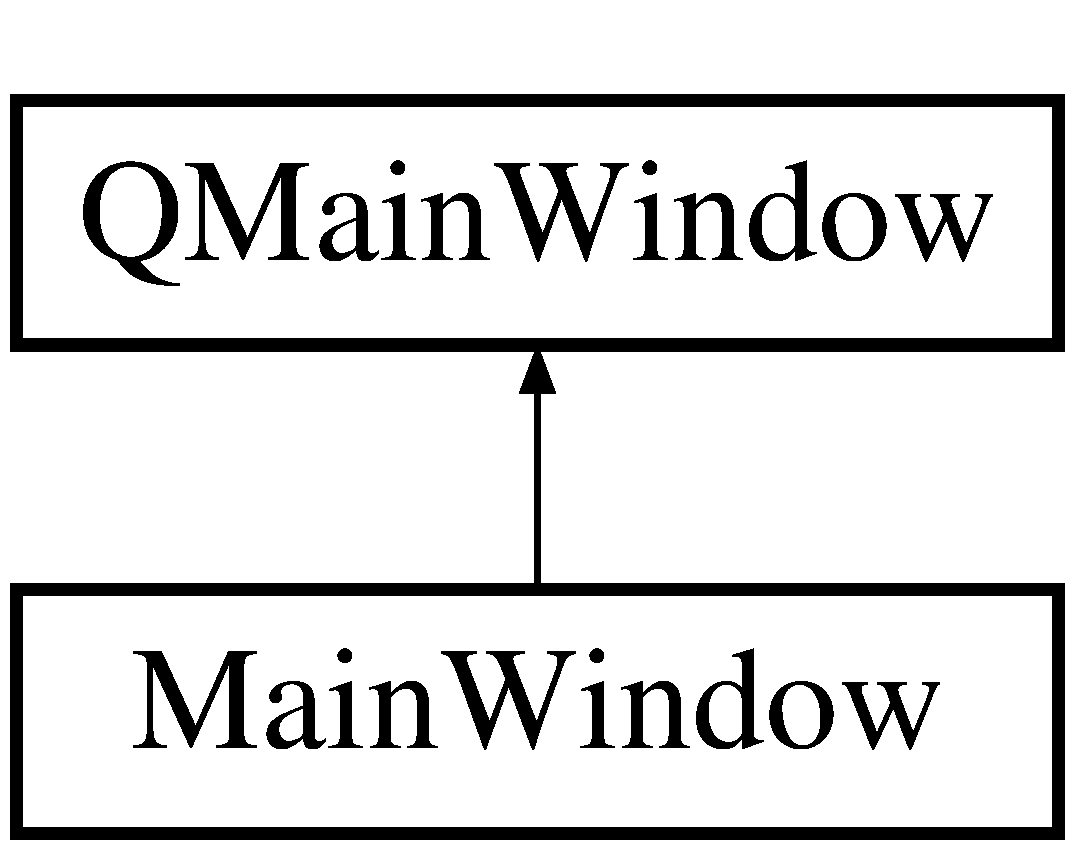
\includegraphics[height=2.000000cm]{class_main_window}
\end{center}
\end{figure}
\subsection*{Public Member Functions}
\begin{DoxyCompactItemize}
\item 
\hypertarget{class_main_window_a8b244be8b7b7db1b08de2a2acb9409db}{}{\bfseries Main\+Window} (Q\+Widget $\ast$parent=0)\label{class_main_window_a8b244be8b7b7db1b08de2a2acb9409db}

\item 
\hypertarget{class_main_window_a0f6f0466e2aca15edd6c820a686c6b57}{}bool {\bfseries painter\+Cursor\+Activated} ()\label{class_main_window_a0f6f0466e2aca15edd6c820a686c6b57}

\item 
\hypertarget{class_main_window_aa0e9c2933778a0a94a2d2010b28ee0f2}{}Q\+Cursor {\bfseries get\+Painter\+Cursor} ()\label{class_main_window_aa0e9c2933778a0a94a2d2010b28ee0f2}

\end{DoxyCompactItemize}
\subsection*{Protected Member Functions}
\begin{DoxyCompactItemize}
\item 
\hypertarget{class_main_window_ae12f8f63791595567b6250f8bb002bda}{}void {\bfseries resize\+Event} (Q\+Resize\+Event $\ast$event)\label{class_main_window_ae12f8f63791595567b6250f8bb002bda}

\end{DoxyCompactItemize}


The documentation for this class was generated from the following files\+:\begin{DoxyCompactItemize}
\item 
Main\+Window.\+h\item 
Main\+Window.\+cpp\end{DoxyCompactItemize}

\hypertarget{class_my_central_ellipse_item}{}\section{My\+Central\+Ellipse\+Item Class Reference}
\label{class_my_central_ellipse_item}\index{My\+Central\+Ellipse\+Item@{My\+Central\+Ellipse\+Item}}
Inheritance diagram for My\+Central\+Ellipse\+Item\+:\begin{figure}[H]
\begin{center}
\leavevmode
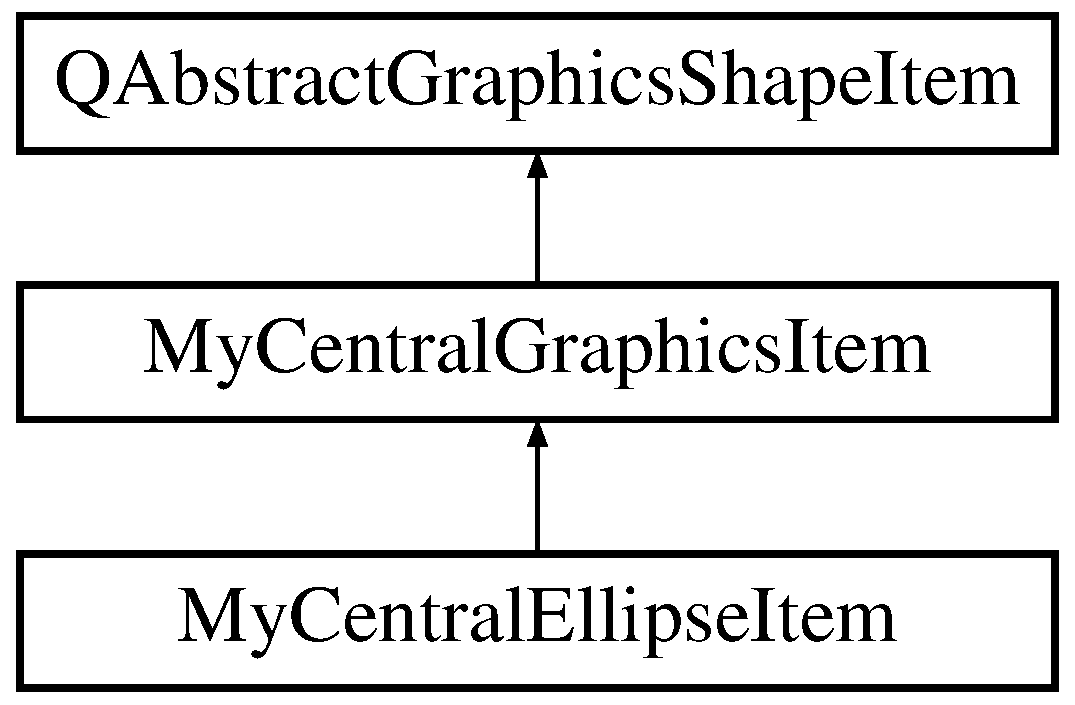
\includegraphics[height=3.000000cm]{class_my_central_ellipse_item}
\end{center}
\end{figure}
\subsection*{Public Member Functions}
\begin{DoxyCompactItemize}
\item 
\hypertarget{class_my_central_ellipse_item_ac912023a16f5f6e6331b1fe861ca42d2}{}{\bfseries My\+Central\+Ellipse\+Item} (const Q\+Rect\+F \&rect, Q\+Graphics\+Item $\ast$parent=0)\label{class_my_central_ellipse_item_ac912023a16f5f6e6331b1fe861ca42d2}

\item 
void \hyperlink{class_my_central_ellipse_item_aa3ae037258cf9839002f8da7e83c3239}{paint} (Q\+Painter $\ast$painter, const Q\+Style\+Option\+Graphics\+Item $\ast$option, Q\+Widget $\ast$widget=0)
\begin{DoxyCompactList}\small\item\em Inherits from \hyperlink{class_my_central_graphics_item}{My\+Central\+Graphics\+Item} to draw the shape of the item. \end{DoxyCompactList}\item 
int \hyperlink{class_my_central_ellipse_item_a94c23343867dce46a608582dfe01fffb}{type} () const 
\item 
Q\+Painter\+Path \hyperlink{class_my_central_ellipse_item_a075835bf21a3d95317ece40e9ca3da7c}{shape} () const 
\item 
Q\+Rect\+F \hyperlink{class_my_central_ellipse_item_a97f879a0bb7cfa7270f33c3d77d5b7a0}{inner\+Rect} ()
\end{DoxyCompactItemize}
\subsection*{Protected Member Functions}
\begin{DoxyCompactItemize}
\item 
void \hyperlink{class_my_central_ellipse_item_ab1b7f9aec994268061b5a38d2cd5744d}{mouse\+Press\+Event} (Q\+Graphics\+Scene\+Mouse\+Event $\ast$event)
\begin{DoxyCompactList}\small\item\em called whenever this item is clicked, inherits from \hyperlink{class_my_central_graphics_item}{My\+Central\+Graphics\+Item} \end{DoxyCompactList}\item 
void \hyperlink{class_my_central_ellipse_item_a0d465a1d4c907bda9d57b3a3207097a9}{hover\+Move\+Event} (Q\+Graphics\+Scene\+Hover\+Event $\ast$event)
\end{DoxyCompactItemize}
\subsection*{Private Types}
\begin{DoxyCompactItemize}
\item 
\hypertarget{class_my_central_ellipse_item_a275b0e7f1c7dd42d1601f29dcaf17ae5}{}enum \{ {\bfseries Type} = 4
 \}\label{class_my_central_ellipse_item_a275b0e7f1c7dd42d1601f29dcaf17ae5}

\begin{DoxyCompactList}\small\item\em Enum type value 4. \end{DoxyCompactList}\end{DoxyCompactItemize}
\subsection*{Additional Inherited Members}


\subsection{Member Function Documentation}
\hypertarget{class_my_central_ellipse_item_a0d465a1d4c907bda9d57b3a3207097a9}{}\index{My\+Central\+Ellipse\+Item@{My\+Central\+Ellipse\+Item}!hover\+Move\+Event@{hover\+Move\+Event}}
\index{hover\+Move\+Event@{hover\+Move\+Event}!My\+Central\+Ellipse\+Item@{My\+Central\+Ellipse\+Item}}
\subsubsection[{hover\+Move\+Event}]{\setlength{\rightskip}{0pt plus 5cm}void My\+Central\+Ellipse\+Item\+::hover\+Move\+Event (
\begin{DoxyParamCaption}
\item[{Q\+Graphics\+Scene\+Hover\+Event $\ast$}]{event}
\end{DoxyParamCaption}
)\hspace{0.3cm}{\ttfamily [protected]}}\label{class_my_central_ellipse_item_a0d465a1d4c907bda9d57b3a3207097a9}
The Hover event has to be used since, instead of the boundingrect corners of the ellipse, we will use the inner rect corners to resize de ellipse. So that when the user hovers over the inner conners the current cursor changes the shape indicating that he can press and resize the ellipse \hypertarget{class_my_central_ellipse_item_a97f879a0bb7cfa7270f33c3d77d5b7a0}{}\index{My\+Central\+Ellipse\+Item@{My\+Central\+Ellipse\+Item}!inner\+Rect@{inner\+Rect}}
\index{inner\+Rect@{inner\+Rect}!My\+Central\+Ellipse\+Item@{My\+Central\+Ellipse\+Item}}
\subsubsection[{inner\+Rect}]{\setlength{\rightskip}{0pt plus 5cm}Q\+Rect\+F My\+Central\+Ellipse\+Item\+::inner\+Rect (
\begin{DoxyParamCaption}
{}
\end{DoxyParamCaption}
)}\label{class_my_central_ellipse_item_a97f879a0bb7cfa7270f33c3d77d5b7a0}
\hyperlink{class_my_central_ellipse_item_a97f879a0bb7cfa7270f33c3d77d5b7a0}{inner\+Rect()} is used to return the inner rectangle in the ellipse. \hypertarget{class_my_central_ellipse_item_ab1b7f9aec994268061b5a38d2cd5744d}{}\index{My\+Central\+Ellipse\+Item@{My\+Central\+Ellipse\+Item}!mouse\+Press\+Event@{mouse\+Press\+Event}}
\index{mouse\+Press\+Event@{mouse\+Press\+Event}!My\+Central\+Ellipse\+Item@{My\+Central\+Ellipse\+Item}}
\subsubsection[{mouse\+Press\+Event}]{\setlength{\rightskip}{0pt plus 5cm}void My\+Central\+Ellipse\+Item\+::mouse\+Press\+Event (
\begin{DoxyParamCaption}
\item[{Q\+Graphics\+Scene\+Mouse\+Event $\ast$}]{event}
\end{DoxyParamCaption}
)\hspace{0.3cm}{\ttfamily [protected]}}\label{class_my_central_ellipse_item_ab1b7f9aec994268061b5a38d2cd5744d}


called whenever this item is clicked, inherits from \hyperlink{class_my_central_graphics_item}{My\+Central\+Graphics\+Item} 


\begin{DoxyParams}{Parameters}
{\em event} & used to get the position of the cursor when this function is called \\
\hline
\end{DoxyParams}
If the painter\+Cursor is activated, then this item color should be changed.

This part is different from My\+Central\+Graphics\+Item\+::mouse\+Press\+Event() since I have to use the inner rectangle, instead of the bounding rectangle check \hyperlink{class_my_central_ellipse_item_ab1b7f9aec994268061b5a38d2cd5744d}{mouse\+Press\+Event()} in My\+Central\+Graphics\+Item.\+cpp to see the difference in the following if statements\hypertarget{class_my_central_ellipse_item_aa3ae037258cf9839002f8da7e83c3239}{}\index{My\+Central\+Ellipse\+Item@{My\+Central\+Ellipse\+Item}!paint@{paint}}
\index{paint@{paint}!My\+Central\+Ellipse\+Item@{My\+Central\+Ellipse\+Item}}
\subsubsection[{paint}]{\setlength{\rightskip}{0pt plus 5cm}void My\+Central\+Ellipse\+Item\+::paint (
\begin{DoxyParamCaption}
\item[{Q\+Painter $\ast$}]{painter, }
\item[{const Q\+Style\+Option\+Graphics\+Item $\ast$}]{option, }
\item[{Q\+Widget $\ast$}]{widget = {\ttfamily 0}}
\end{DoxyParamCaption}
)}\label{class_my_central_ellipse_item_aa3ae037258cf9839002f8da7e83c3239}


Inherits from \hyperlink{class_my_central_graphics_item}{My\+Central\+Graphics\+Item} to draw the shape of the item. 

Called whenever there is a change in this Item (resize, move, etc). Used to draw the ellipse on the bounding\+Rect(). \hypertarget{class_my_central_ellipse_item_a075835bf21a3d95317ece40e9ca3da7c}{}\index{My\+Central\+Ellipse\+Item@{My\+Central\+Ellipse\+Item}!shape@{shape}}
\index{shape@{shape}!My\+Central\+Ellipse\+Item@{My\+Central\+Ellipse\+Item}}
\subsubsection[{shape}]{\setlength{\rightskip}{0pt plus 5cm}Q\+Painter\+Path My\+Central\+Ellipse\+Item\+::shape (
\begin{DoxyParamCaption}
{}
\end{DoxyParamCaption}
) const}\label{class_my_central_ellipse_item_a075835bf21a3d95317ece40e9ca3da7c}
\hyperlink{class_my_central_ellipse_item_a075835bf21a3d95317ece40e9ca3da7c}{shape()} was supposed to be used to get the intersection point with the line that was connecting this Item, but isnt really used since I couldnt move the beginning point of the line to the porder of the ellipse, so I had to paint the background with white. Setting the Z value of the line lower than the z value of this item \hypertarget{class_my_central_ellipse_item_a94c23343867dce46a608582dfe01fffb}{}\index{My\+Central\+Ellipse\+Item@{My\+Central\+Ellipse\+Item}!type@{type}}
\index{type@{type}!My\+Central\+Ellipse\+Item@{My\+Central\+Ellipse\+Item}}
\subsubsection[{type}]{\setlength{\rightskip}{0pt plus 5cm}int My\+Central\+Ellipse\+Item\+::type (
\begin{DoxyParamCaption}
{}
\end{DoxyParamCaption}
) const\hspace{0.3cm}{\ttfamily [inline]}, {\ttfamily [virtual]}}\label{class_my_central_ellipse_item_a94c23343867dce46a608582dfe01fffb}
\hyperlink{class_my_central_ellipse_item_a94c23343867dce46a608582dfe01fffb}{type()} will be used to get the type of item I am dropping into \hyperlink{class_my_drop_graphics_scene}{My\+Drop\+Graphics\+Scene} or in some other ocassions when you dont know which item is which 

Implements \hyperlink{class_my_central_graphics_item}{My\+Central\+Graphics\+Item}.



The documentation for this class was generated from the following files\+:\begin{DoxyCompactItemize}
\item 
My\+Central\+Ellipse\+Item.\+h\item 
My\+Central\+Ellipse\+Item.\+cpp\end{DoxyCompactItemize}

\hypertarget{class_my_central_graphics_item}{}\section{My\+Central\+Graphics\+Item Class Reference}
\label{class_my_central_graphics_item}\index{My\+Central\+Graphics\+Item@{My\+Central\+Graphics\+Item}}
Inheritance diagram for My\+Central\+Graphics\+Item\+:\begin{figure}[H]
\begin{center}
\leavevmode
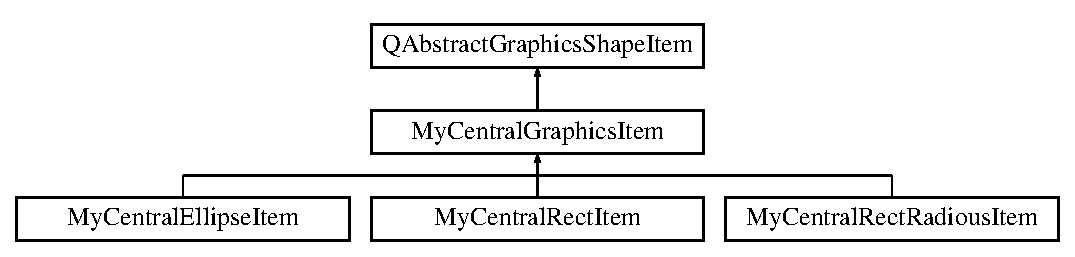
\includegraphics[height=3.000000cm]{class_my_central_graphics_item}
\end{center}
\end{figure}
\subsection*{Public Member Functions}
\begin{DoxyCompactItemize}
\item 
\hypertarget{class_my_central_graphics_item_aad8e57045bd2fa779167b03cc4d904f6}{}{\bfseries My\+Central\+Graphics\+Item} (const Q\+Rect\+F \&rect, Q\+Graphics\+Item $\ast$parent=0)\label{class_my_central_graphics_item_aad8e57045bd2fa779167b03cc4d904f6}

\item 
\hypertarget{class_my_central_graphics_item_a7f7865060c07eb7f53de607b96af4374}{}void {\bfseries paint} (Q\+Painter $\ast$painter, const Q\+Style\+Option\+Graphics\+Item $\ast$option, Q\+Widget $\ast$widget=0)\label{class_my_central_graphics_item_a7f7865060c07eb7f53de607b96af4374}

\item 
\hypertarget{class_my_central_graphics_item_a4b6fb53c59a68427af7b50d87e575b55}{}Q\+Rect\+F {\bfseries bounding\+Rect} () const \label{class_my_central_graphics_item_a4b6fb53c59a68427af7b50d87e575b55}

\item 
\hypertarget{class_my_central_graphics_item_a5cf920e7f80b31b6c1b7584f9b69644a}{}Q\+Point\+F $\ast$ {\bfseries up} ()\label{class_my_central_graphics_item_a5cf920e7f80b31b6c1b7584f9b69644a}

\item 
\hypertarget{class_my_central_graphics_item_a2fb024ca79a6058a3e1b57e8503b07f1}{}Q\+Point\+F $\ast$ {\bfseries down} ()\label{class_my_central_graphics_item_a2fb024ca79a6058a3e1b57e8503b07f1}

\item 
\hypertarget{class_my_central_graphics_item_a464f64aaceac539ed3cd7340ec78be23}{}Q\+Point\+F $\ast$ {\bfseries right} ()\label{class_my_central_graphics_item_a464f64aaceac539ed3cd7340ec78be23}

\item 
\hypertarget{class_my_central_graphics_item_a00cbf493f2486086609589d70cc5ba07}{}Q\+Point\+F $\ast$ {\bfseries left} ()\label{class_my_central_graphics_item_a00cbf493f2486086609589d70cc5ba07}

\item 
\hypertarget{class_my_central_graphics_item_afe51dd4af5f6a9f0d7f9724fd447cf15}{}double {\bfseries top\+Right\+Angle} ()\label{class_my_central_graphics_item_afe51dd4af5f6a9f0d7f9724fd447cf15}

\item 
\hypertarget{class_my_central_graphics_item_ab2e87f4e08a71e5457495777658f3acd}{}double {\bfseries top\+Left\+Angle} ()\label{class_my_central_graphics_item_ab2e87f4e08a71e5457495777658f3acd}

\item 
\hypertarget{class_my_central_graphics_item_a2f7682741d279d241f1918ce0481bf76}{}double {\bfseries bottom\+Right\+Angle} ()\label{class_my_central_graphics_item_a2f7682741d279d241f1918ce0481bf76}

\item 
\hypertarget{class_my_central_graphics_item_a00dac82c3de7ac8e4c82b6a67640fc96}{}double {\bfseries bottom\+Left\+Angle} ()\label{class_my_central_graphics_item_a00dac82c3de7ac8e4c82b6a67640fc96}

\item 
\hypertarget{class_my_central_graphics_item_a69d74fc2be942bba5724001725da7a20}{}virtual int {\bfseries type} () const =0\label{class_my_central_graphics_item_a69d74fc2be942bba5724001725da7a20}

\item 
\hypertarget{class_my_central_graphics_item_ab8c895264ea2bbfae7cd4be206450919}{}Q\+Cursor {\bfseries get\+Painter\+Cursor} ()\label{class_my_central_graphics_item_ab8c895264ea2bbfae7cd4be206450919}

\end{DoxyCompactItemize}
\subsection*{Protected Member Functions}
\begin{DoxyCompactItemize}
\item 
\hypertarget{class_my_central_graphics_item_a37c26b04ff0579568550e479aca6b4c7}{}void {\bfseries hover\+Move\+Event} (Q\+Graphics\+Scene\+Hover\+Event $\ast$event)\label{class_my_central_graphics_item_a37c26b04ff0579568550e479aca6b4c7}

\item 
\hypertarget{class_my_central_graphics_item_ac2eca49285c8f2058c8faab20ec46b48}{}void {\bfseries mouse\+Press\+Event} (Q\+Graphics\+Scene\+Mouse\+Event $\ast$event)\label{class_my_central_graphics_item_ac2eca49285c8f2058c8faab20ec46b48}

\item 
\hypertarget{class_my_central_graphics_item_a6b3c312c410910a45e0883e728312f3c}{}void {\bfseries mouse\+Move\+Event} (Q\+Graphics\+Scene\+Mouse\+Event $\ast$event)\label{class_my_central_graphics_item_a6b3c312c410910a45e0883e728312f3c}

\item 
\hypertarget{class_my_central_graphics_item_aa0d27bc8f661136a54a61e12d79e2386}{}bool {\bfseries verify\+Corner} (const Q\+Point\+F \&p1, const Q\+Point\+F \&p2)\label{class_my_central_graphics_item_aa0d27bc8f661136a54a61e12d79e2386}

\item 
\hypertarget{class_my_central_graphics_item_a7616ccc14383191dd0c69a0a3b3e4e2c}{}int {\bfseries resize\+Mode} () const \label{class_my_central_graphics_item_a7616ccc14383191dd0c69a0a3b3e4e2c}

\item 
\hypertarget{class_my_central_graphics_item_a37551f69c8e31e601036ceef0cc16a40}{}void {\bfseries set\+Resize\+Mode} (int i)\label{class_my_central_graphics_item_a37551f69c8e31e601036ceef0cc16a40}

\item 
\hypertarget{class_my_central_graphics_item_a3b8c5b13546c1f1e9eba541abe1aa89c}{}void {\bfseries update\+Connecting\+Points} ()\label{class_my_central_graphics_item_a3b8c5b13546c1f1e9eba541abe1aa89c}

\end{DoxyCompactItemize}
\subsection*{Protected Attributes}
\begin{DoxyCompactItemize}
\item 
\hypertarget{class_my_central_graphics_item_a64d9cd163863d34aa141ce8103dd8ec0}{}Q\+Pen $\ast$ {\bfseries pen}\label{class_my_central_graphics_item_a64d9cd163863d34aa141ce8103dd8ec0}

\end{DoxyCompactItemize}
\subsection*{Private Member Functions}
\begin{DoxyCompactItemize}
\item 
\hypertarget{class_my_central_graphics_item_a15879cd62e4ed70768e75f9e8f6c64d5}{}void {\bfseries connect\+Scene} ()\label{class_my_central_graphics_item_a15879cd62e4ed70768e75f9e8f6c64d5}

\end{DoxyCompactItemize}
\subsection*{Private Attributes}
\begin{DoxyCompactItemize}
\item 
\hypertarget{class_my_central_graphics_item_a1c3c6f131281480fdc3a8958eef3f2e8}{}int {\bfseries r\+Mode}\label{class_my_central_graphics_item_a1c3c6f131281480fdc3a8958eef3f2e8}

\item 
\hypertarget{class_my_central_graphics_item_afbe7a635f347c8ce75f2f194ea3a987d}{}Q\+Point\+F {\bfseries closest\+Point}\label{class_my_central_graphics_item_afbe7a635f347c8ce75f2f194ea3a987d}

\item 
\hypertarget{class_my_central_graphics_item_af93bfde444b10668aabe20622a83fe8c}{}Q\+Rect\+F {\bfseries rect}\label{class_my_central_graphics_item_af93bfde444b10668aabe20622a83fe8c}

\item 
\hypertarget{class_my_central_graphics_item_a9b7eaf6b7cd651197d685c36d973554f}{}Q\+Cursor {\bfseries painter\+Cursor}\label{class_my_central_graphics_item_a9b7eaf6b7cd651197d685c36d973554f}

\item 
\hypertarget{class_my_central_graphics_item_a9a4a2166b5975fc43679722640c55599}{}Q\+Point\+F {\bfseries p\+Up}\label{class_my_central_graphics_item_a9a4a2166b5975fc43679722640c55599}

\item 
\hypertarget{class_my_central_graphics_item_a8e98a25b3f2e6088d6a003d62a89207b}{}Q\+Point\+F {\bfseries p\+Down}\label{class_my_central_graphics_item_a8e98a25b3f2e6088d6a003d62a89207b}

\item 
\hypertarget{class_my_central_graphics_item_ae2db19506332f5717da9dd9dd5856c07}{}Q\+Point\+F {\bfseries p\+Right}\label{class_my_central_graphics_item_ae2db19506332f5717da9dd9dd5856c07}

\item 
\hypertarget{class_my_central_graphics_item_a8efbd0c513117cd1e773d91770fee899}{}Q\+Point\+F {\bfseries p\+Left}\label{class_my_central_graphics_item_a8efbd0c513117cd1e773d91770fee899}

\end{DoxyCompactItemize}


The documentation for this class was generated from the following files\+:\begin{DoxyCompactItemize}
\item 
My\+Central\+Graphics\+Item.\+h\item 
My\+Central\+Graphics\+Item.\+cpp\end{DoxyCompactItemize}

\hypertarget{class_my_central_rect_item}{}\section{My\+Central\+Rect\+Item Class Reference}
\label{class_my_central_rect_item}\index{My\+Central\+Rect\+Item@{My\+Central\+Rect\+Item}}
Inheritance diagram for My\+Central\+Rect\+Item\+:\begin{figure}[H]
\begin{center}
\leavevmode
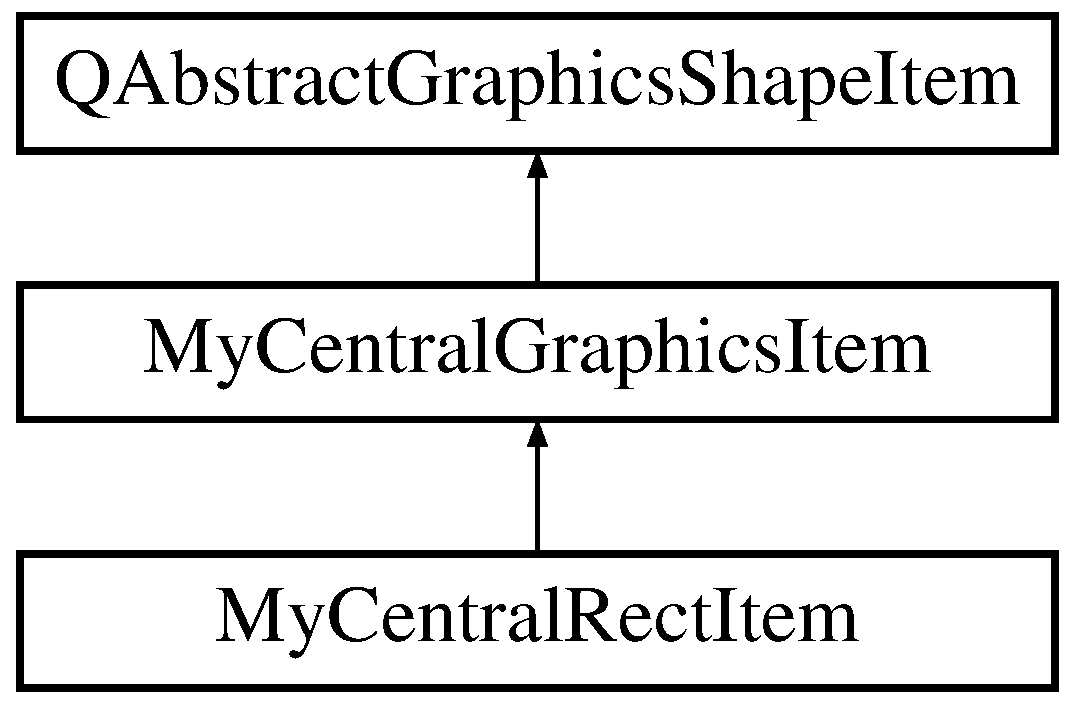
\includegraphics[height=3.000000cm]{class_my_central_rect_item}
\end{center}
\end{figure}
\subsection*{Public Member Functions}
\begin{DoxyCompactItemize}
\item 
\hypertarget{class_my_central_rect_item_a7edf24741fb0098e78dea7079d2983f3}{}{\bfseries My\+Central\+Rect\+Item} (const Q\+Rect\+F \&rect, Q\+Graphics\+Item $\ast$parent=0)\label{class_my_central_rect_item_a7edf24741fb0098e78dea7079d2983f3}

\item 
\hypertarget{class_my_central_rect_item_a87c70071f69fb8fc4142af545447f326}{}void {\bfseries paint} (Q\+Painter $\ast$painter, const Q\+Style\+Option\+Graphics\+Item $\ast$option, Q\+Widget $\ast$widget=0)\label{class_my_central_rect_item_a87c70071f69fb8fc4142af545447f326}

\item 
\hypertarget{class_my_central_rect_item_a4b970e08db43fd6b8f18dce8114458c2}{}int {\bfseries type} () const \label{class_my_central_rect_item_a4b970e08db43fd6b8f18dce8114458c2}

\end{DoxyCompactItemize}
\subsection*{Protected Member Functions}
\begin{DoxyCompactItemize}
\item 
\hypertarget{class_my_central_rect_item_ac6ed556955ad6f3c2643311e3de22f7a}{}void {\bfseries mouse\+Press\+Event} (Q\+Graphics\+Scene\+Mouse\+Event $\ast$event)\label{class_my_central_rect_item_ac6ed556955ad6f3c2643311e3de22f7a}

\end{DoxyCompactItemize}
\subsection*{Private Types}
\begin{DoxyCompactItemize}
\item 
\hypertarget{class_my_central_rect_item_a9ef9aaf375a9e9d809aff54511e926da}{}enum \{ {\bfseries Type} = 1
 \}\label{class_my_central_rect_item_a9ef9aaf375a9e9d809aff54511e926da}

\end{DoxyCompactItemize}
\subsection*{Additional Inherited Members}


The documentation for this class was generated from the following files\+:\begin{DoxyCompactItemize}
\item 
My\+Central\+Rect\+Item.\+h\item 
My\+Central\+Rect\+Item.\+cpp\end{DoxyCompactItemize}

\hypertarget{class_my_central_rect_radious_item}{}\section{My\+Central\+Rect\+Radious\+Item Class Reference}
\label{class_my_central_rect_radious_item}\index{My\+Central\+Rect\+Radious\+Item@{My\+Central\+Rect\+Radious\+Item}}
Inheritance diagram for My\+Central\+Rect\+Radious\+Item\+:\begin{figure}[H]
\begin{center}
\leavevmode
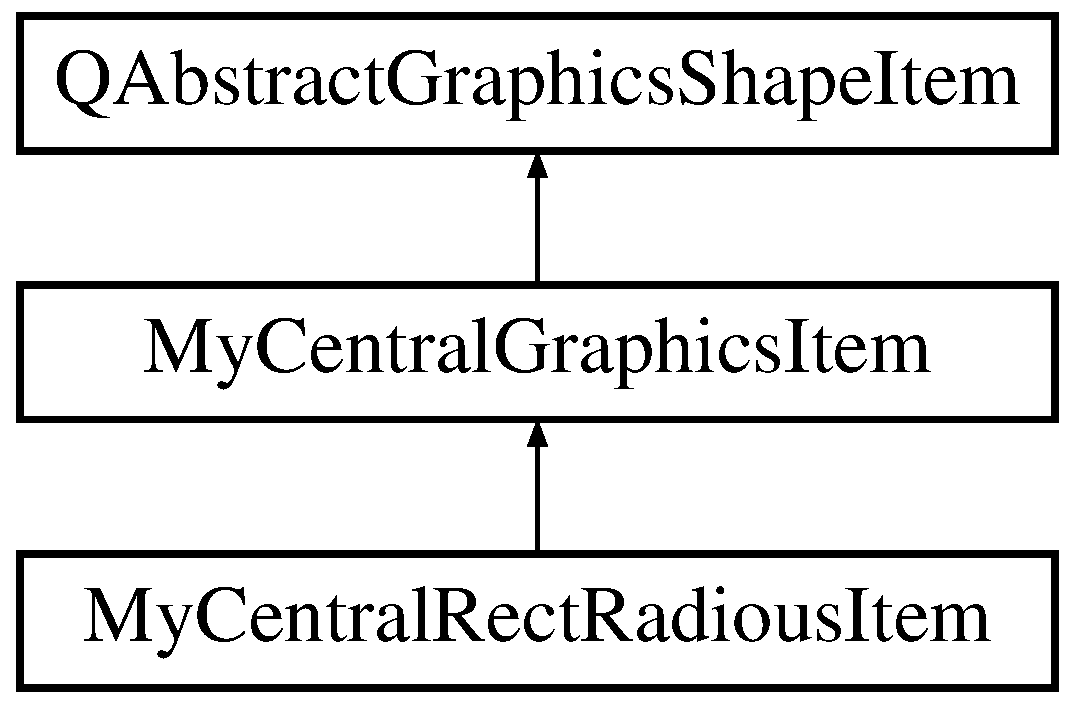
\includegraphics[height=3.000000cm]{class_my_central_rect_radious_item}
\end{center}
\end{figure}
\subsection*{Public Member Functions}
\begin{DoxyCompactItemize}
\item 
\hypertarget{class_my_central_rect_radious_item_a746f17b384cddf85069bf50ef573de02}{}{\bfseries My\+Central\+Rect\+Radious\+Item} (const Q\+Rect\+F \&rect, Q\+Graphics\+Item $\ast$parent=0)\label{class_my_central_rect_radious_item_a746f17b384cddf85069bf50ef573de02}

\item 
\hypertarget{class_my_central_rect_radious_item_a6169e6c0d0a4736311fbc531abd4069e}{}void {\bfseries paint} (Q\+Painter $\ast$painter, const Q\+Style\+Option\+Graphics\+Item $\ast$option, Q\+Widget $\ast$widget=0)\label{class_my_central_rect_radious_item_a6169e6c0d0a4736311fbc531abd4069e}

\item 
\hypertarget{class_my_central_rect_radious_item_a1910592e03509484118253aed0ed8142}{}int {\bfseries type} () const \label{class_my_central_rect_radious_item_a1910592e03509484118253aed0ed8142}

\end{DoxyCompactItemize}
\subsection*{Protected Member Functions}
\begin{DoxyCompactItemize}
\item 
\hypertarget{class_my_central_rect_radious_item_aaf825576276007052dbbb3f21e2c71b8}{}void {\bfseries mouse\+Press\+Event} (Q\+Graphics\+Scene\+Mouse\+Event $\ast$event)\label{class_my_central_rect_radious_item_aaf825576276007052dbbb3f21e2c71b8}

\end{DoxyCompactItemize}
\subsection*{Additional Inherited Members}


The documentation for this class was generated from the following files\+:\begin{DoxyCompactItemize}
\item 
My\+Central\+Rect\+Radious\+Item.\+h\item 
My\+Central\+Rect\+Radious\+Item.\+cpp\end{DoxyCompactItemize}

\hypertarget{class_my_dock_text_item}{}\section{My\+Dock\+Text\+Item Class Reference}
\label{class_my_dock_text_item}\index{My\+Dock\+Text\+Item@{My\+Dock\+Text\+Item}}
Inheritance diagram for My\+Dock\+Text\+Item\+:\begin{figure}[H]
\begin{center}
\leavevmode
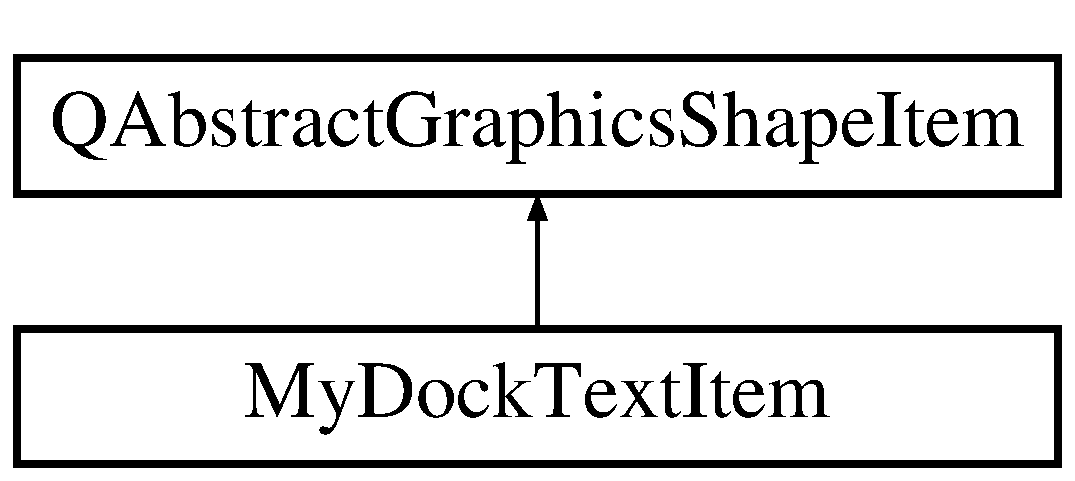
\includegraphics[height=2.000000cm]{class_my_dock_text_item}
\end{center}
\end{figure}
\subsection*{Public Types}
\begin{DoxyCompactItemize}
\item 
\hypertarget{class_my_dock_text_item_a074d30a5cf2cabd19ce476cac37f6e84}{}enum \{ {\bfseries Type} = 5
 \}\label{class_my_dock_text_item_a074d30a5cf2cabd19ce476cac37f6e84}

\end{DoxyCompactItemize}
\subsection*{Public Member Functions}
\begin{DoxyCompactItemize}
\item 
\hypertarget{class_my_dock_text_item_a6cf92df4f4166fc82922edba23b4d887}{}{\bfseries My\+Dock\+Text\+Item} (const Q\+Rect\+F \&rect, Q\+Graphics\+Item $\ast$parent=0)\label{class_my_dock_text_item_a6cf92df4f4166fc82922edba23b4d887}

\item 
\hypertarget{class_my_dock_text_item_a121a427a41555d6395a6201577c2026b}{}int {\bfseries type} () const \label{class_my_dock_text_item_a121a427a41555d6395a6201577c2026b}

\item 
\hypertarget{class_my_dock_text_item_a68218bef6c0945e5bf3499b6a824c200}{}void {\bfseries paint} (Q\+Painter $\ast$painter, const Q\+Style\+Option\+Graphics\+Item $\ast$option, Q\+Widget $\ast$widget=0)\label{class_my_dock_text_item_a68218bef6c0945e5bf3499b6a824c200}

\item 
\hypertarget{class_my_dock_text_item_aa44a1ed17c5db699fd3e1ef62d432edc}{}Q\+Rect\+F {\bfseries bounding\+Rect} () const \label{class_my_dock_text_item_aa44a1ed17c5db699fd3e1ef62d432edc}

\end{DoxyCompactItemize}
\subsection*{Protected Member Functions}
\begin{DoxyCompactItemize}
\item 
\hypertarget{class_my_dock_text_item_a2948d3050a83589e02305a85022ef3e7}{}void {\bfseries mouse\+Press\+Event} (Q\+Graphics\+Scene\+Mouse\+Event $\ast$event)\label{class_my_dock_text_item_a2948d3050a83589e02305a85022ef3e7}

\end{DoxyCompactItemize}
\subsection*{Protected Attributes}
\begin{DoxyCompactItemize}
\item 
\hypertarget{class_my_dock_text_item_a8cb7660e2e72b8318a9365dbfbc8998e}{}Q\+Drag $\ast$ {\bfseries drag}\label{class_my_dock_text_item_a8cb7660e2e72b8318a9365dbfbc8998e}

\end{DoxyCompactItemize}


The documentation for this class was generated from the following files\+:\begin{DoxyCompactItemize}
\item 
My\+Dock\+Text\+Item.\+h\item 
My\+Dock\+Text\+Item.\+cpp\end{DoxyCompactItemize}

\hypertarget{class_my_drop_graphics_scene}{}\section{My\+Drop\+Graphics\+Scene Class Reference}
\label{class_my_drop_graphics_scene}\index{My\+Drop\+Graphics\+Scene@{My\+Drop\+Graphics\+Scene}}
Inheritance diagram for My\+Drop\+Graphics\+Scene\+:\begin{figure}[H]
\begin{center}
\leavevmode
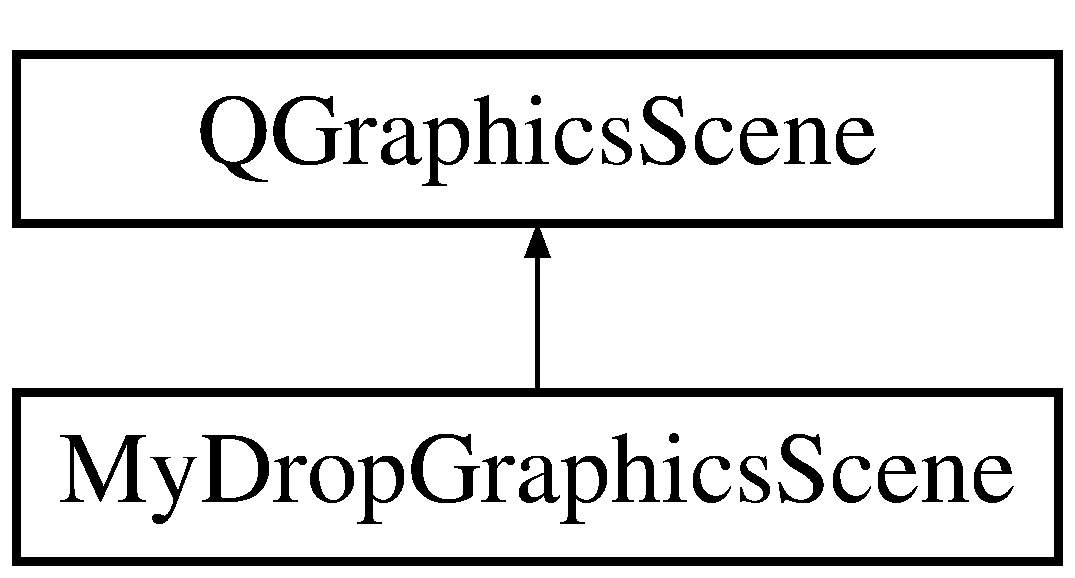
\includegraphics[height=2.000000cm]{class_my_drop_graphics_scene}
\end{center}
\end{figure}
\subsection*{Public Member Functions}
\begin{DoxyCompactItemize}
\item 
\hypertarget{class_my_drop_graphics_scene_a4f001c01ee3f40b7d7e41fbb7c93a42f}{}{\bfseries My\+Drop\+Graphics\+Scene} (Q\+Object $\ast$parent=0)\label{class_my_drop_graphics_scene_a4f001c01ee3f40b7d7e41fbb7c93a42f}

\item 
\hypertarget{class_my_drop_graphics_scene_a07c494016c9c30715f5c34e499448415}{}void {\bfseries connect} ()\label{class_my_drop_graphics_scene_a07c494016c9c30715f5c34e499448415}

\item 
\hypertarget{class_my_drop_graphics_scene_a692183e5780c07b03bf82398a6c585c6}{}Q\+List$<$ \hyperlink{class_my_central_graphics_item}{My\+Central\+Graphics\+Item} $\ast$ $>$ {\bfseries items} () const \label{class_my_drop_graphics_scene_a692183e5780c07b03bf82398a6c585c6}

\item 
\hypertarget{class_my_drop_graphics_scene_ab3153d2dde7fce4b850b933a973d3a67}{}double {\bfseries distance} (const \hyperlink{class_my_point_f}{My\+Point\+F} $\ast$p1, const \hyperlink{class_my_point_f}{My\+Point\+F} $\ast$p2) const \label{class_my_drop_graphics_scene_ab3153d2dde7fce4b850b933a973d3a67}

\item 
\hypertarget{class_my_drop_graphics_scene_acbfa92a87bc4177817c2549ec3ad0b67}{}void {\bfseries add\+Item} (Q\+Graphics\+Item $\ast$item)\label{class_my_drop_graphics_scene_acbfa92a87bc4177817c2549ec3ad0b67}

\item 
\hypertarget{class_my_drop_graphics_scene_a812d93b88a1179d99306b5b58b2e3a08}{}void {\bfseries set\+Painter\+Color} (Q\+Color color)\label{class_my_drop_graphics_scene_a812d93b88a1179d99306b5b58b2e3a08}

\item 
\hypertarget{class_my_drop_graphics_scene_ac2dac4faf1c3ba9f6358b470397ab249}{}Q\+Color {\bfseries painter\+Color} ()\label{class_my_drop_graphics_scene_ac2dac4faf1c3ba9f6358b470397ab249}

\item 
\hypertarget{class_my_drop_graphics_scene_a49e4e26f0864b0ba20221689b49c654b}{}void {\bfseries remove\+Item} (Q\+Graphics\+Item $\ast$item)\label{class_my_drop_graphics_scene_a49e4e26f0864b0ba20221689b49c654b}

\end{DoxyCompactItemize}
\subsection*{Protected Member Functions}
\begin{DoxyCompactItemize}
\item 
\hypertarget{class_my_drop_graphics_scene_a1a5dd8b0ac8aa55645d1d8c919451350}{}void {\bfseries drop\+Event} (Q\+Graphics\+Scene\+Drag\+Drop\+Event $\ast$event)\label{class_my_drop_graphics_scene_a1a5dd8b0ac8aa55645d1d8c919451350}

\item 
\hypertarget{class_my_drop_graphics_scene_a050aa1d5a7861ad4f320da82219a63d2}{}void {\bfseries drag\+Enter\+Event} (Q\+Graphics\+Scene\+Drag\+Drop\+Event $\ast$event)\label{class_my_drop_graphics_scene_a050aa1d5a7861ad4f320da82219a63d2}

\item 
\hypertarget{class_my_drop_graphics_scene_a407f26d50aa080e00f1097ffee0f41ce}{}void {\bfseries drag\+Move\+Event} (Q\+Graphics\+Scene\+Drag\+Drop\+Event $\ast$event)\label{class_my_drop_graphics_scene_a407f26d50aa080e00f1097ffee0f41ce}

\item 
\hypertarget{class_my_drop_graphics_scene_a856ec4eddc556b20abf3831b0ca3910a}{}void {\bfseries key\+Press\+Event} (Q\+Key\+Event $\ast$event)\label{class_my_drop_graphics_scene_a856ec4eddc556b20abf3831b0ca3910a}

\item 
\hypertarget{class_my_drop_graphics_scene_af8d211f3518dcc347f80eaebfee8a09a}{}bool {\bfseries event} (Q\+Event $\ast$event)\label{class_my_drop_graphics_scene_af8d211f3518dcc347f80eaebfee8a09a}

\end{DoxyCompactItemize}
\subsection*{Private Member Functions}
\begin{DoxyCompactItemize}
\item 
\hypertarget{class_my_drop_graphics_scene_ade89f2b11675821eec338ffdcff948f5}{}void {\bfseries reduce\+Line\+To\+Borders} (Q\+Line\+F \&, \hyperlink{class_my_point_f}{My\+Point\+F} $\ast$, int)\label{class_my_drop_graphics_scene_ade89f2b11675821eec338ffdcff948f5}

\end{DoxyCompactItemize}
\subsection*{Private Attributes}
\begin{DoxyCompactItemize}
\item 
\hypertarget{class_my_drop_graphics_scene_ac7085f0aaf1b342d91c554a842c000e5}{}Q\+List$<$ \hyperlink{class_my_central_graphics_item}{My\+Central\+Graphics\+Item} $\ast$ $>$ {\bfseries my\+Items}\label{class_my_drop_graphics_scene_ac7085f0aaf1b342d91c554a842c000e5}

\item 
\hypertarget{class_my_drop_graphics_scene_a5d0b65a8d6b76bd9f0e951aa0b7bc81f}{}Q\+List$<$ Q\+Graphics\+Line\+Item $\ast$ $>$ {\bfseries lines\+List}\label{class_my_drop_graphics_scene_a5d0b65a8d6b76bd9f0e951aa0b7bc81f}

\item 
\hypertarget{class_my_drop_graphics_scene_ae483c253389eb08913a0b906653d2e31}{}Q\+Color $\ast$ {\bfseries paintercolor}\label{class_my_drop_graphics_scene_ae483c253389eb08913a0b906653d2e31}

\end{DoxyCompactItemize}


The documentation for this class was generated from the following files\+:\begin{DoxyCompactItemize}
\item 
My\+Drop\+Graphics\+Scene.\+h\item 
My\+Drop\+Graphics\+Scene.\+cpp\end{DoxyCompactItemize}

\hypertarget{class_my_ellipse_item}{}\section{My\+Ellipse\+Item Class Reference}
\label{class_my_ellipse_item}\index{My\+Ellipse\+Item@{My\+Ellipse\+Item}}
Inheritance diagram for My\+Ellipse\+Item\+:\begin{figure}[H]
\begin{center}
\leavevmode
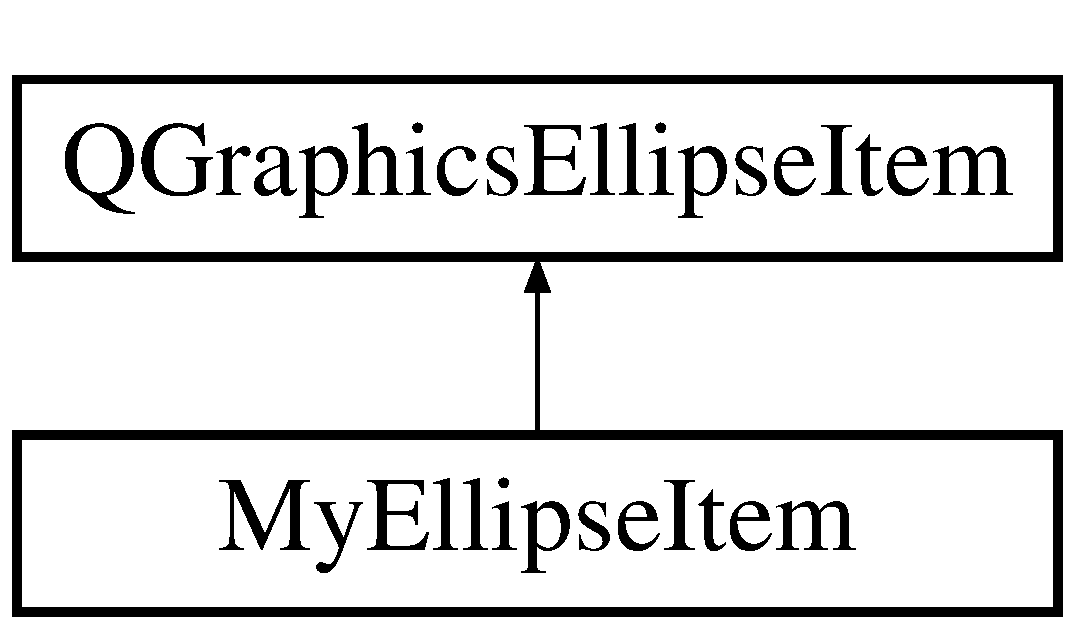
\includegraphics[height=2.000000cm]{class_my_ellipse_item}
\end{center}
\end{figure}
\subsection*{Public Types}
\begin{DoxyCompactItemize}
\item 
\hypertarget{class_my_ellipse_item_ab3d7ea5bd2ccd432ae8969dc1f733edc}{}enum \{ {\bfseries Type} = 4
 \}\label{class_my_ellipse_item_ab3d7ea5bd2ccd432ae8969dc1f733edc}

\end{DoxyCompactItemize}
\subsection*{Public Member Functions}
\begin{DoxyCompactItemize}
\item 
\hypertarget{class_my_ellipse_item_a781d85f2fdfd5a843cb28bc67993b228}{}{\bfseries My\+Ellipse\+Item} (const Q\+Rect\+F \&rect, Q\+Graphics\+Item $\ast$parent=0)\label{class_my_ellipse_item_a781d85f2fdfd5a843cb28bc67993b228}

\item 
\hypertarget{class_my_ellipse_item_a7188e1d0368309413fcc30e8e528bed9}{}int {\bfseries type} () const \label{class_my_ellipse_item_a7188e1d0368309413fcc30e8e528bed9}

\end{DoxyCompactItemize}
\subsection*{Protected Member Functions}
\begin{DoxyCompactItemize}
\item 
\hypertarget{class_my_ellipse_item_a0ead6a18fca86196833f8d7fbd225ee5}{}void {\bfseries mouse\+Press\+Event} (Q\+Graphics\+Scene\+Mouse\+Event $\ast$event)\label{class_my_ellipse_item_a0ead6a18fca86196833f8d7fbd225ee5}

\end{DoxyCompactItemize}
\subsection*{Protected Attributes}
\begin{DoxyCompactItemize}
\item 
\hypertarget{class_my_ellipse_item_a70624351d663b438ec225b3cb0eba7d9}{}Q\+Drag $\ast$ {\bfseries drag}\label{class_my_ellipse_item_a70624351d663b438ec225b3cb0eba7d9}

\end{DoxyCompactItemize}


The documentation for this class was generated from the following files\+:\begin{DoxyCompactItemize}
\item 
My\+Ellipse\+Item.\+h\item 
My\+Ellipse\+Item.\+cpp\end{DoxyCompactItemize}

\hypertarget{class_my_graphics_view}{}\section{My\+Graphics\+View Class Reference}
\label{class_my_graphics_view}\index{My\+Graphics\+View@{My\+Graphics\+View}}
Inheritance diagram for My\+Graphics\+View\+:\begin{figure}[H]
\begin{center}
\leavevmode
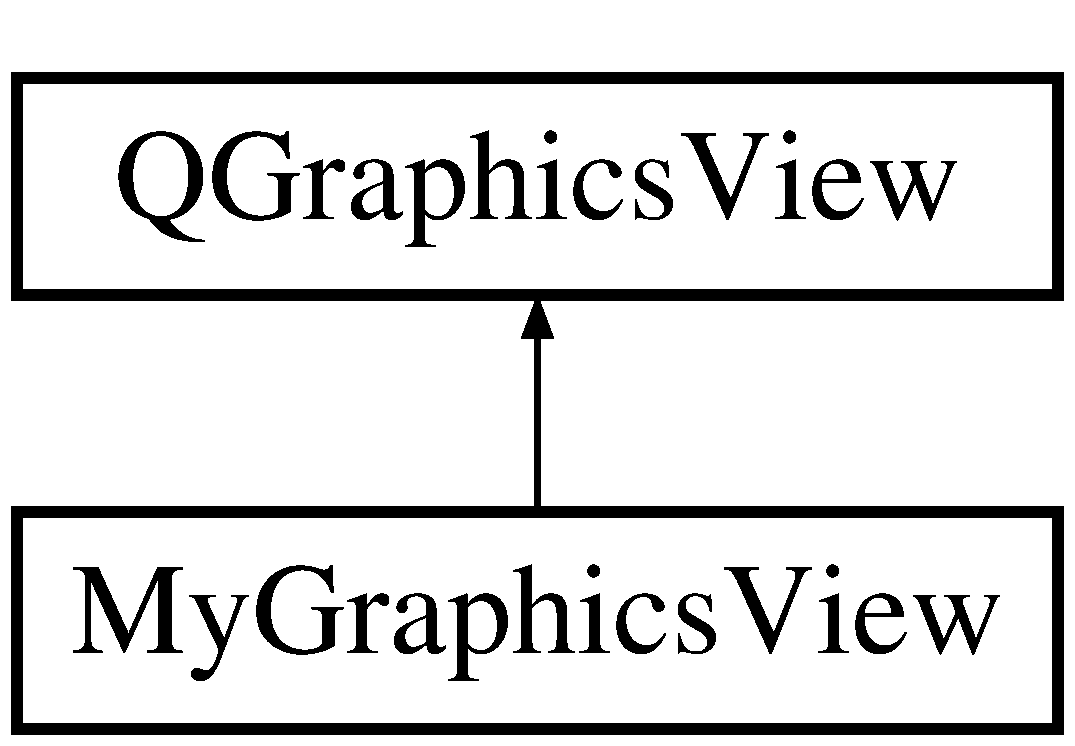
\includegraphics[height=2.000000cm]{class_my_graphics_view}
\end{center}
\end{figure}
\subsection*{Public Member Functions}
\begin{DoxyCompactItemize}
\item 
\hypertarget{class_my_graphics_view_a7236beae467bc43ed9f88222b25d4874}{}{\bfseries My\+Graphics\+View} (\hyperlink{class_my_drop_graphics_scene}{My\+Drop\+Graphics\+Scene} $\ast$scene, Q\+Widget $\ast$parent=0)\label{class_my_graphics_view_a7236beae467bc43ed9f88222b25d4874}

\end{DoxyCompactItemize}
\subsection*{Protected Member Functions}
\begin{DoxyCompactItemize}
\item 
\hypertarget{class_my_graphics_view_a22dd9a814c979d818ab322706f0b9297}{}void {\bfseries drag\+Enter\+Event} (Q\+Drag\+Enter\+Event $\ast$event)\label{class_my_graphics_view_a22dd9a814c979d818ab322706f0b9297}

\item 
\hypertarget{class_my_graphics_view_a7c1982f74cf31f7d2b5721e16ed5587a}{}void {\bfseries drag\+Leave\+Event} (Q\+Drag\+Leave\+Event $\ast$event)\label{class_my_graphics_view_a7c1982f74cf31f7d2b5721e16ed5587a}

\item 
\hypertarget{class_my_graphics_view_a3c475cb56178cd729b97fce19008ffe9}{}void {\bfseries drag\+Move\+Event} (Q\+Drag\+Move\+Event $\ast$event)\label{class_my_graphics_view_a3c475cb56178cd729b97fce19008ffe9}

\item 
\hypertarget{class_my_graphics_view_a26906e53c7aa71c8ade8067e98de90b3}{}void {\bfseries drop\+Event} (Q\+Drop\+Event $\ast$event)\label{class_my_graphics_view_a26906e53c7aa71c8ade8067e98de90b3}

\end{DoxyCompactItemize}
\subsection*{Private Attributes}
\begin{DoxyCompactItemize}
\item 
\hypertarget{class_my_graphics_view_a96bd1f2147b155a6efb1e407e5784200}{}\hyperlink{class_my_drop_graphics_scene}{My\+Drop\+Graphics\+Scene} $\ast$ {\bfseries Scene}\label{class_my_graphics_view_a96bd1f2147b155a6efb1e407e5784200}

\end{DoxyCompactItemize}


The documentation for this class was generated from the following files\+:\begin{DoxyCompactItemize}
\item 
My\+Graphics\+View.\+h\item 
My\+Graphics\+View.\+cpp\end{DoxyCompactItemize}

\hypertarget{class_my_organization_dock_widget}{}\section{My\+Organization\+Dock\+Widget Class Reference}
\label{class_my_organization_dock_widget}\index{My\+Organization\+Dock\+Widget@{My\+Organization\+Dock\+Widget}}
Inheritance diagram for My\+Organization\+Dock\+Widget\+:\begin{figure}[H]
\begin{center}
\leavevmode
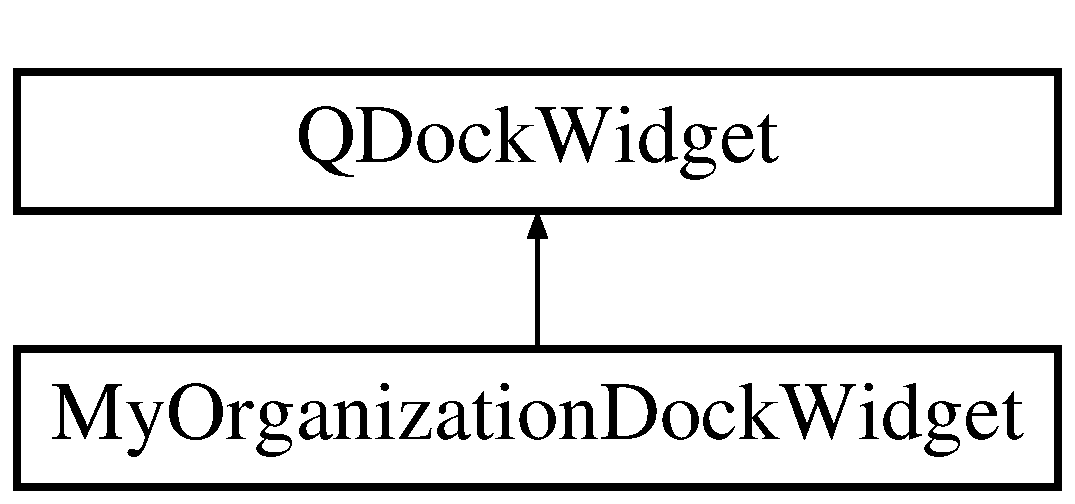
\includegraphics[height=2.000000cm]{class_my_organization_dock_widget}
\end{center}
\end{figure}
\subsection*{Public Member Functions}
\begin{DoxyCompactItemize}
\item 
\hypertarget{class_my_organization_dock_widget_aac6c63cd09ef063f95872800c400666a}{}{\bfseries My\+Organization\+Dock\+Widget} (const Q\+String \&title, Q\+Widget $\ast$parent=0, Qt\+::\+Window\+Flags flags=0)\label{class_my_organization_dock_widget_aac6c63cd09ef063f95872800c400666a}

\end{DoxyCompactItemize}
\subsection*{Protected Member Functions}
\begin{DoxyCompactItemize}
\item 
\hypertarget{class_my_organization_dock_widget_ae2e820b68075f26923adc4b8ff972d1d}{}void {\bfseries resize\+Event} (Q\+Resize\+Event $\ast$event)\label{class_my_organization_dock_widget_ae2e820b68075f26923adc4b8ff972d1d}

\end{DoxyCompactItemize}


The documentation for this class was generated from the following files\+:\begin{DoxyCompactItemize}
\item 
My\+Organization\+Dock\+Widget.\+h\item 
My\+Organization\+Dock\+Widget.\+cpp\end{DoxyCompactItemize}

\hypertarget{class_my_point_f}{}\section{My\+Point\+F Class Reference}
\label{class_my_point_f}\index{My\+Point\+F@{My\+Point\+F}}
Inheritance diagram for My\+Point\+F\+:\begin{figure}[H]
\begin{center}
\leavevmode
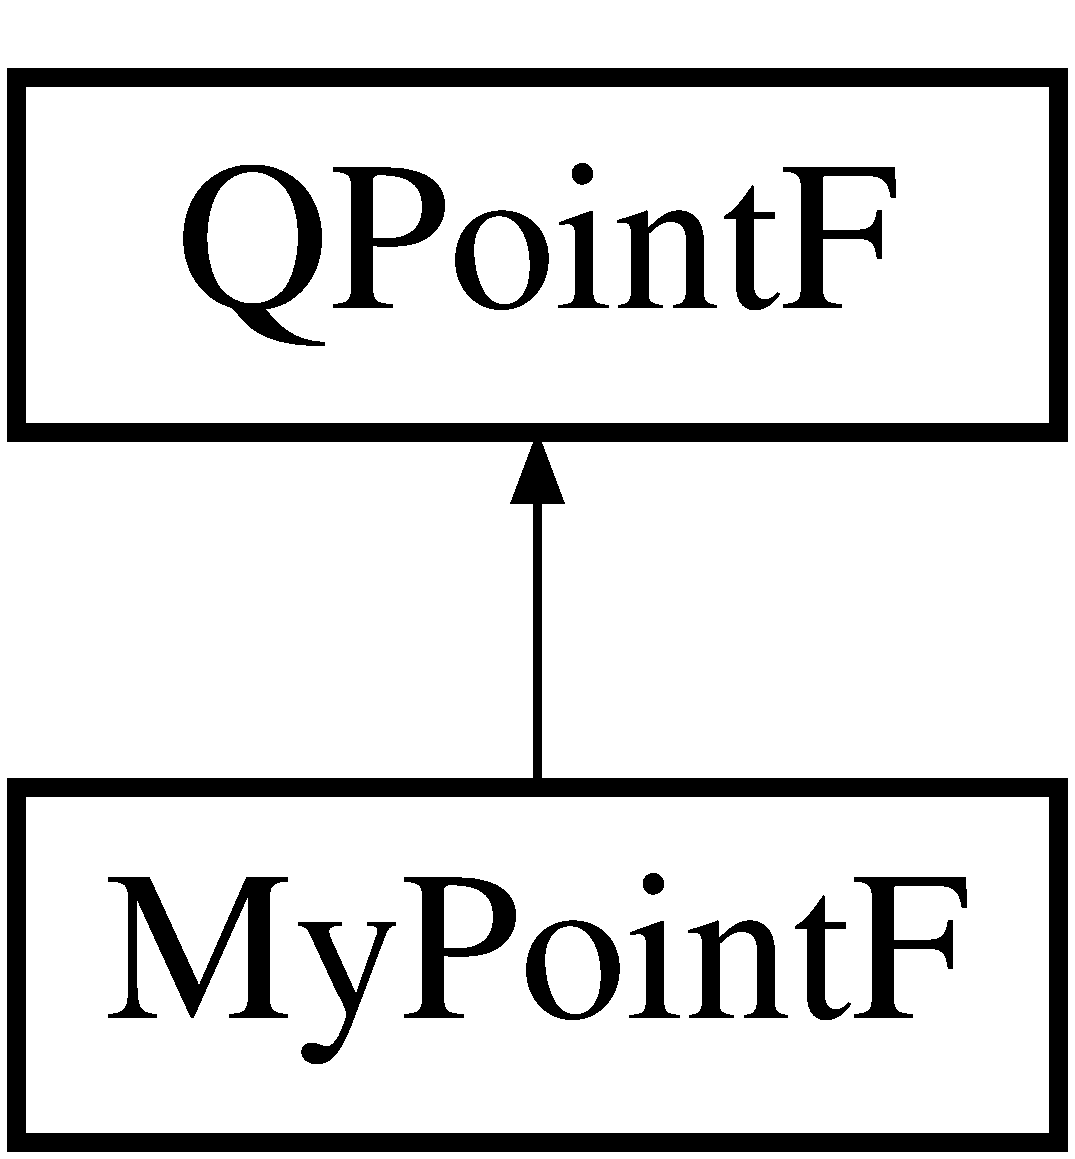
\includegraphics[height=2.000000cm]{class_my_point_f}
\end{center}
\end{figure}
\subsection*{Public Attributes}
\begin{DoxyCompactItemize}
\item 
\hypertarget{class_my_point_f_ad38dddef3e72005d48fac561eaf0fd15}{}Q\+Graphics\+Line\+Item $\ast$ {\bfseries connecting\+Line}\label{class_my_point_f_ad38dddef3e72005d48fac561eaf0fd15}

\item 
\hypertarget{class_my_point_f_a61bd27efc4a2001e5db086e8eba61636}{}Q\+Graphics\+Item $\ast$ {\bfseries item}\label{class_my_point_f_a61bd27efc4a2001e5db086e8eba61636}

\item 
\hypertarget{class_my_point_f_a5206b8bcf9a21c12c9649c21c54e204a}{}\hyperlink{class_my_point_f}{My\+Point\+F} $\ast$ {\bfseries closest\+Point}\label{class_my_point_f_a5206b8bcf9a21c12c9649c21c54e204a}

\item 
\hypertarget{class_my_point_f_a310cc7f9bf6abc5fc5c068aaf1f2c4a0}{}double {\bfseries closest\+Distance}\label{class_my_point_f_a310cc7f9bf6abc5fc5c068aaf1f2c4a0}

\end{DoxyCompactItemize}


The documentation for this class was generated from the following file\+:\begin{DoxyCompactItemize}
\item 
My\+Point\+F.\+h\end{DoxyCompactItemize}

\hypertarget{class_my_rect_item}{}\section{My\+Rect\+Item Class Reference}
\label{class_my_rect_item}\index{My\+Rect\+Item@{My\+Rect\+Item}}
Inheritance diagram for My\+Rect\+Item\+:\begin{figure}[H]
\begin{center}
\leavevmode
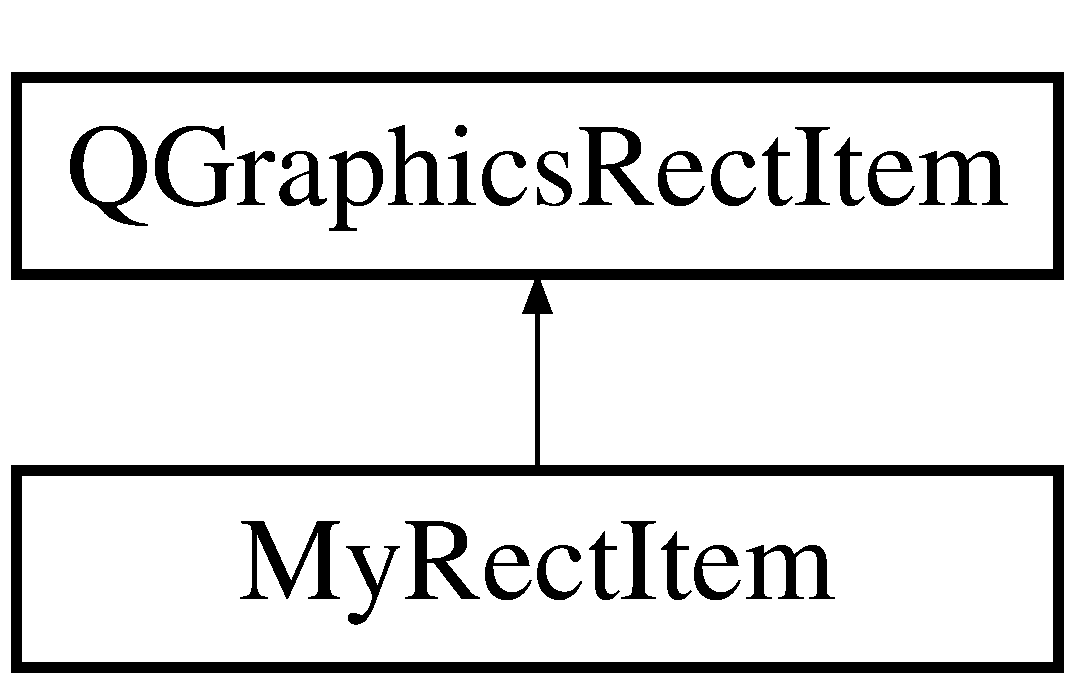
\includegraphics[height=2.000000cm]{class_my_rect_item}
\end{center}
\end{figure}
\subsection*{Public Types}
\begin{DoxyCompactItemize}
\item 
\hypertarget{class_my_rect_item_a7c879c8fc50d7da6e36405d8a55688e1}{}enum \{ {\bfseries Type} = 1
 \}\label{class_my_rect_item_a7c879c8fc50d7da6e36405d8a55688e1}

\end{DoxyCompactItemize}
\subsection*{Public Member Functions}
\begin{DoxyCompactItemize}
\item 
\hypertarget{class_my_rect_item_adb1987c24d2977cde750e98c9f34b801}{}{\bfseries My\+Rect\+Item} (const Q\+Rect\+F \&rect, Q\+Graphics\+Item $\ast$parent=0)\label{class_my_rect_item_adb1987c24d2977cde750e98c9f34b801}

\item 
\hypertarget{class_my_rect_item_a5392f7adb9afeb5fb1de90424b1d25ed}{}int {\bfseries type} () const \label{class_my_rect_item_a5392f7adb9afeb5fb1de90424b1d25ed}

\end{DoxyCompactItemize}
\subsection*{Protected Member Functions}
\begin{DoxyCompactItemize}
\item 
\hypertarget{class_my_rect_item_a6fe4b88e45e42f693e101bd35372721f}{}void {\bfseries mouse\+Press\+Event} (Q\+Graphics\+Scene\+Mouse\+Event $\ast$event)\label{class_my_rect_item_a6fe4b88e45e42f693e101bd35372721f}

\end{DoxyCompactItemize}
\subsection*{Protected Attributes}
\begin{DoxyCompactItemize}
\item 
\hypertarget{class_my_rect_item_a9d38187add8c23b7de77e8870293833b}{}Q\+Drag $\ast$ {\bfseries drag}\label{class_my_rect_item_a9d38187add8c23b7de77e8870293833b}

\end{DoxyCompactItemize}


The documentation for this class was generated from the following files\+:\begin{DoxyCompactItemize}
\item 
My\+Rect\+Item.\+h\item 
My\+Rect\+Item.\+cpp\end{DoxyCompactItemize}

\hypertarget{class_my_rect_radious_item}{}\section{My\+Rect\+Radious\+Item Class Reference}
\label{class_my_rect_radious_item}\index{My\+Rect\+Radious\+Item@{My\+Rect\+Radious\+Item}}
Inheritance diagram for My\+Rect\+Radious\+Item\+:\begin{figure}[H]
\begin{center}
\leavevmode
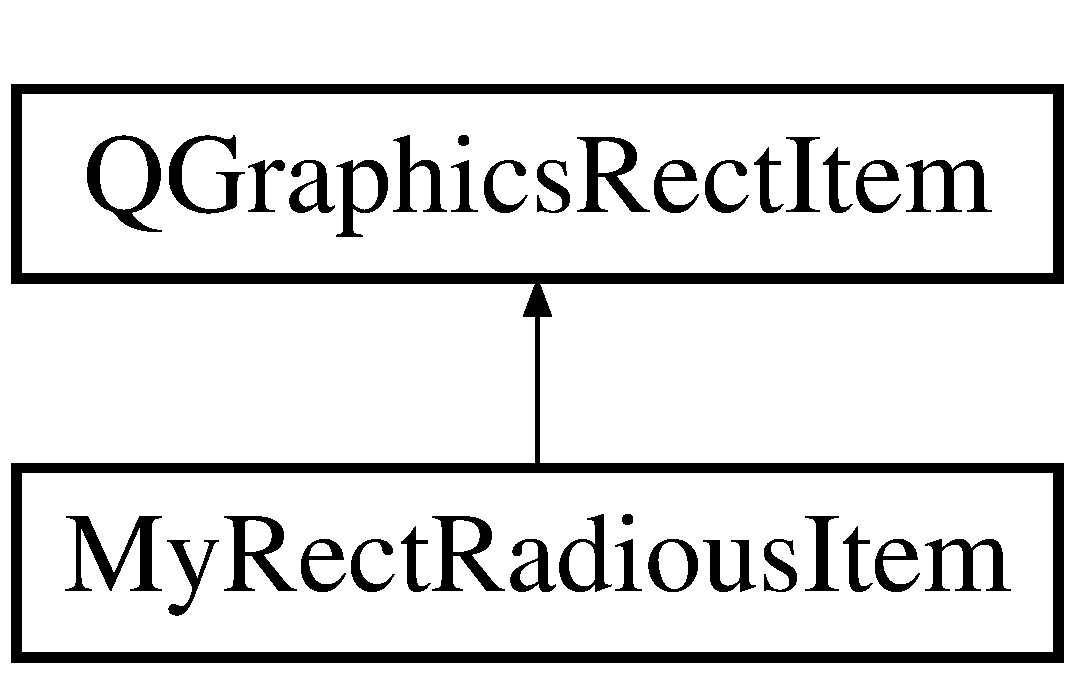
\includegraphics[height=2.000000cm]{class_my_rect_radious_item}
\end{center}
\end{figure}
\subsection*{Public Types}
\begin{DoxyCompactItemize}
\item 
\hypertarget{class_my_rect_radious_item_afbf4ec490ddfd44216fdb7bb063449c1}{}enum \{ {\bfseries Type} = 2
 \}\label{class_my_rect_radious_item_afbf4ec490ddfd44216fdb7bb063449c1}

\end{DoxyCompactItemize}
\subsection*{Public Member Functions}
\begin{DoxyCompactItemize}
\item 
\hypertarget{class_my_rect_radious_item_ac967dc8ad5a9913a531e40ef62c97a17}{}{\bfseries My\+Rect\+Radious\+Item} (const Q\+Rect\+F \&rect, Q\+Graphics\+Item $\ast$parent=0)\label{class_my_rect_radious_item_ac967dc8ad5a9913a531e40ef62c97a17}

\item 
\hypertarget{class_my_rect_radious_item_a7a05b62d804aa0e8d8c4d71c74a2c0e1}{}int {\bfseries type} () const \label{class_my_rect_radious_item_a7a05b62d804aa0e8d8c4d71c74a2c0e1}

\item 
\hypertarget{class_my_rect_radious_item_a395db98794d9637fb4313b0dc1076bca}{}void {\bfseries paint} (Q\+Painter $\ast$painter, const Q\+Style\+Option\+Graphics\+Item $\ast$option, Q\+Widget $\ast$widget=0)\label{class_my_rect_radious_item_a395db98794d9637fb4313b0dc1076bca}

\end{DoxyCompactItemize}
\subsection*{Protected Member Functions}
\begin{DoxyCompactItemize}
\item 
\hypertarget{class_my_rect_radious_item_ad28af1823cfa410b78718837a78edb6c}{}void {\bfseries mouse\+Press\+Event} (Q\+Graphics\+Scene\+Mouse\+Event $\ast$event)\label{class_my_rect_radious_item_ad28af1823cfa410b78718837a78edb6c}

\end{DoxyCompactItemize}
\subsection*{Protected Attributes}
\begin{DoxyCompactItemize}
\item 
\hypertarget{class_my_rect_radious_item_ae3a3010697b291fc7fe1bcac243d1d99}{}Q\+Drag $\ast$ {\bfseries drag}\label{class_my_rect_radious_item_ae3a3010697b291fc7fe1bcac243d1d99}

\end{DoxyCompactItemize}


The documentation for this class was generated from the following files\+:\begin{DoxyCompactItemize}
\item 
My\+Rect\+Radious\+Item.\+h\item 
My\+Rect\+Radious\+Item.\+cpp\end{DoxyCompactItemize}

\hypertarget{class_my_simple_text_item}{}\section{My\+Simple\+Text\+Item Class Reference}
\label{class_my_simple_text_item}\index{My\+Simple\+Text\+Item@{My\+Simple\+Text\+Item}}
Inheritance diagram for My\+Simple\+Text\+Item\+:\begin{figure}[H]
\begin{center}
\leavevmode
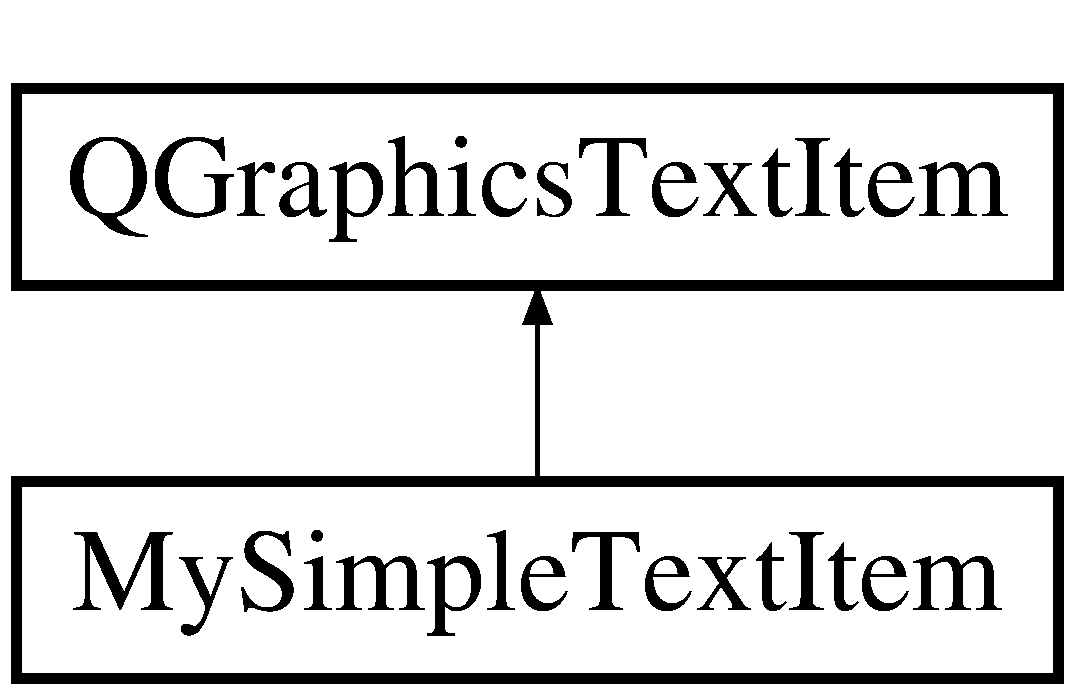
\includegraphics[height=2.000000cm]{class_my_simple_text_item}
\end{center}
\end{figure}
\subsection*{Public Member Functions}
\begin{DoxyCompactItemize}
\item 
\hypertarget{class_my_simple_text_item_abcb188d82eae8c094d053c30f414e5f7}{}{\bfseries My\+Simple\+Text\+Item} (const Q\+String \&text, Q\+Graphics\+Item $\ast$parent=0)\label{class_my_simple_text_item_abcb188d82eae8c094d053c30f414e5f7}

\item 
\hypertarget{class_my_simple_text_item_acdb1382024e54a67c89b887b5ec67f47}{}int {\bfseries type} () const \label{class_my_simple_text_item_acdb1382024e54a67c89b887b5ec67f47}

\item 
\hypertarget{class_my_simple_text_item_a470357b08ba50dff3c95934f75be294c}{}void {\bfseries paint} (Q\+Painter $\ast$painter, const Q\+Style\+Option\+Graphics\+Item $\ast$option, Q\+Widget $\ast$widget)\label{class_my_simple_text_item_a470357b08ba50dff3c95934f75be294c}

\end{DoxyCompactItemize}
\subsection*{Private Types}
\begin{DoxyCompactItemize}
\item 
\hypertarget{class_my_simple_text_item_a6483b53c725f5e46bc9e9ba16ee909e3}{}enum \{ {\bfseries Type} = 5
 \}\label{class_my_simple_text_item_a6483b53c725f5e46bc9e9ba16ee909e3}

\end{DoxyCompactItemize}


The documentation for this class was generated from the following files\+:\begin{DoxyCompactItemize}
\item 
My\+Simple\+Text\+Item.\+h\item 
My\+Simple\+Text\+Item.\+cpp\end{DoxyCompactItemize}

%--- End generated contents ---

% Index
\backmatter
\newpage
\phantomsection
\clearemptydoublepage
\addcontentsline{toc}{chapter}{Index}
\printindex

\end{document}
